\documentclass{beamer}

\usepackage{rbstyle}
\usepackage{listings}
\usepackage[utf8]{inputenc}


\title{Big Data}
\subtitle{Projekt: Amazon-Reviews}
\author[Nameshort]{Matthias Körschens \& Kevin Reinke}
\institute{Friedrich-Schiller-Universität Jena}

\newfontfamily\Consolas{Consolas}
\lstset{basicstyle=\small\Consolas} 

\begin{document}
	\nofooter{
		\frame{\titlepage}
	}
	\begin{frame}
		\frametitle{Inhalt}
		\tableofcontents
	\end{frame}
	\section{Zielsetzung}
	\begin{frame}
	\frametitle{Ziel}
	\begin{itemize}
		\item Explorative Datenanalyse von Amazon-Reviews
		\item Im Speziellen:
		\begin{itemize}
			\item Verteilung der Reviews
			\item Bewertungsverhalten der Nutzer
			\item Clustern von Nutzern
		\end{itemize}
	\end{itemize}
	\end{frame}
	\section{Datensatz}
	\begin{frame}
	\framesubsection{Allgemeines}
	\begin{itemize}
	\item AmazonReviews von \url{http://jmcauley.ucsd.edu/data/amazon/}
	\item Zeitraum: Mai 1996 bis Juni 2014
	\item Teildatensatz: Elektronik
	\item 4,7 GB
	\item 7,8 Millionen Reviews und etwa 4,2 Millionen Nutzern
	\item Format: JSON
	\end{itemize}
	\end{frame}
	\begin{frame}[containsverbatim]
	\framesubsection{Beispiel}
	\begin{lstlisting}[breaklines=true]
{ 
  "reviewerID": "A2SUAM1J3GNN3B", 
  "asin": "0000013714", 
  "reviewerName": "J. McDonald", 
  "helpful": [2, 3], 
  "reviewText": "I bought this for my husband who plays the piano. He is having a wonderful time playing these old hymns. The music is at times hard to read because we think the book was published for singing from more than playing from. Great purchase though!", 
  "overall": 5.0, 
  "summary": "Heavenly Highway Hymns", 
  "unixReviewTime": 1252800000, 
  "reviewTime": "09 13, 2009" 
}
	\end{lstlisting}  
	\end{frame}
	\section{Strukturen}
	\begin{frame}
	\subsection{Reviewverteilung nach Reviewanzahl}
	\frametitle{Wie sind die Reviews verteilt?}
	\begin{itemize}
	\item Den Nutzern wurden ihre eigenen Reviews zugeordnet
	\item Viele Nutzer bewerten wenig
	\item 2,88 von 4,2 Millionen Nutzer haben nur ein Review 
	\item Zusammenhang exponentiell (Zipfsches Gesetz)
	\end{itemize}
	\end{frame}
	\frametitle{Wie sind die Reviews verteilt?}	
	\begin{frame}
	\begin{figure}[H]
	\centering
    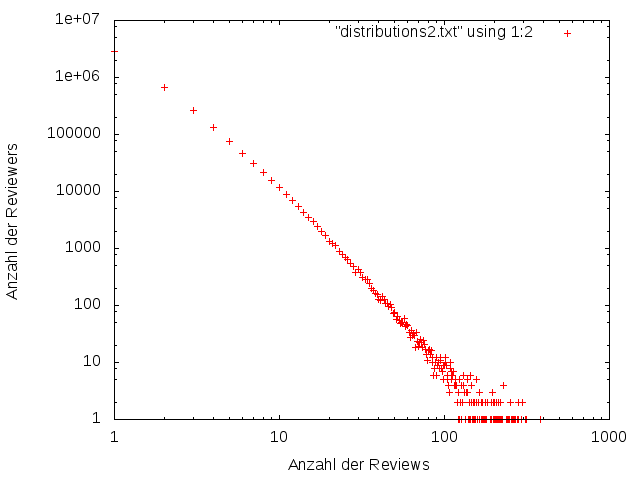
\includegraphics[width=0.8\textwidth]{bild.png}
    \caption{Reviewverteilung}
	\end{figure}
	\end{frame}
	
	\begin{frame}
	\frametitle{Reviewerverhalten bei steigender Reviewanzahl}
	\begin{itemize}
	\item Gruppierung der Nutzer nach Reviewanzahl beibehalten
	\item Merkmale: Bewertung, Wortanzahl, Zeichenanzahl, hilfreich
	\item Innerhalb einer Gruppe Merkmale arithmetisch mitteln
	\end{itemize}
	\end{frame}
	
	\begin{frame}
	\frametitle{Reviewerverhalten bei steigender Reviewanzahl}
	\begin{figure}[H]
\centering
    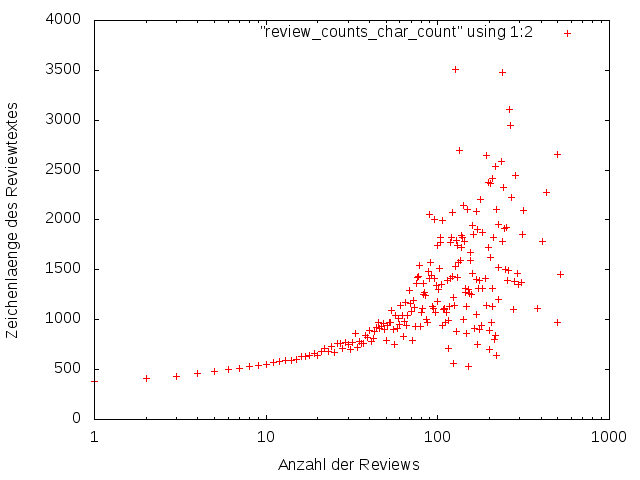
\includegraphics[width=0.8\textwidth]{_results/char_count2.png}
    \caption{Reviewverteilung Reviewanzahl und Zeichenanzahl}
\end{figure}
	\end{frame}
	
		\begin{frame}
	\begin{figure}[H]
\centering
    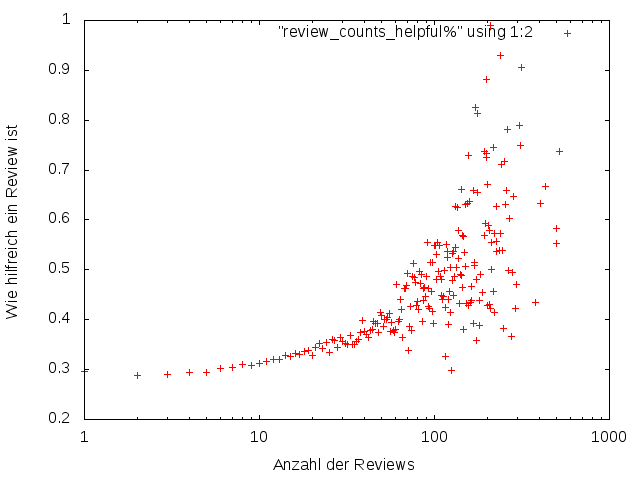
\includegraphics[width=0.8\textwidth]{_results/helpfull_count2.png}
    \caption{Reviewverteilung Reviewanzahl und Hilfreichbewertungen(\%)}
\end{figure}
	\end{frame}
	
		\begin{frame}
	\begin{figure}[H]
\centering
    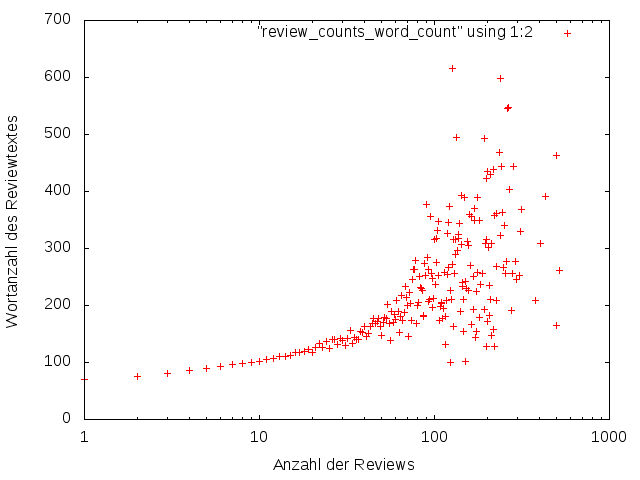
\includegraphics[width=0.8\textwidth]{_results/word_count2.png}
    \caption{Reviewverteilung Reviewanzahl und Wortanzahl}
\end{figure}
	\end{frame}
	
		\begin{frame}
	\begin{figure}[H]
\centering
    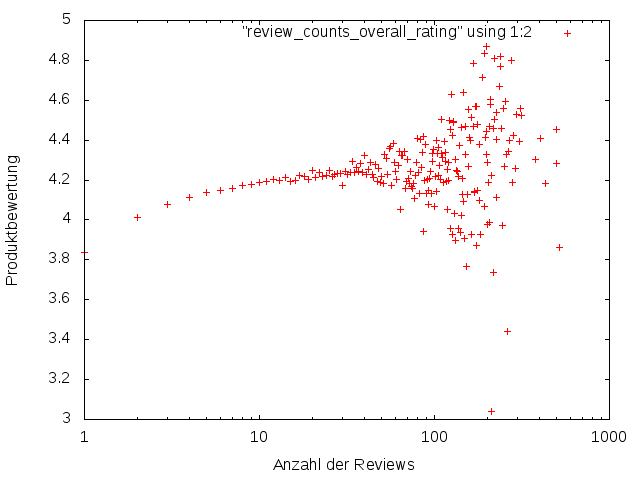
\includegraphics[width=0.8\textwidth]{_results/rating_count.png}
    \caption{Reviewverteilung Reviewanzahl und Produktbewertung}
\end{figure}
	\end{frame}
	
	\begin{frame}
	\subsection{Reviewverteilung nach Textlänge}
	\frametitle{Textlänge und Produktbewertung}
	\begin{itemize}
	\item Analog über Reviewlänge gruppiert
	\item Produktbewertungen je Gruppe gemittelt
	\item Ein Bewertungstief bei ca 180 Wörtern
	\item Ab 1000 Wörtern ungenau
	\end{itemize}
	\end{frame}
		
	\begin{frame}
	\frametitle{Textlänge und Produktbewertung}
	\begin{figure}[H]
    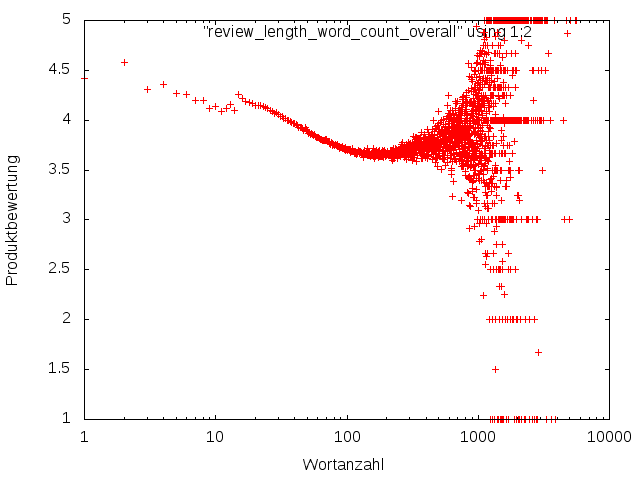
\includegraphics[width=0.8\textwidth]{_results/word_rating.png}
    \caption{Reviewverteilung}
	\end{figure}
	\end{frame}
	
	\begin{frame}
	\frametitle{Textlänge und Produktbewertung}
	\begin{figure}[H]
    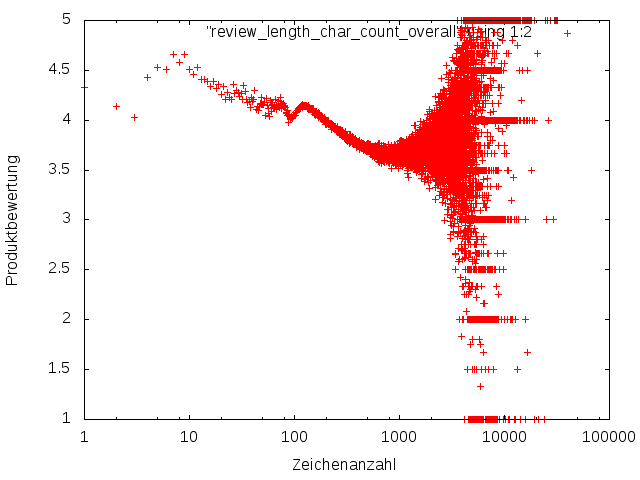
\includegraphics[width=0.8\textwidth]{_results/char_rating.png}
    \caption{Reviewverteilung}
	\end{figure}
	\end{frame}
	
	\section{Clustern}
	\begin{frame}
	\frametitle{Clustering}
	\begin{itemize}
	\item Nutzer mit seinen Reviews erhält Merkmalsvektor
	\item Merkmale:
	\begin{itemize}
	\item Wortanzahl des Bewertungstextes
	\item Zeichenanzahl des Bewertungstextes
	\item Zeitstempel des Reviews
	\item Zeichenanzahl des Reviewtitels
	\item wie hilfreich das Review war prozentual
	\item wieviele das Review ingesamt nützlich fanden
	\item Produktbewertung
	\item Reviewanzahl
	\end{itemize}
	\item Clusterverfahren mit Distanzmaß zwischen allen Reviewern $\rightarrow$ verworfen, da zu aufwändig
	\item PCA
	\item K-Means mit $k=2,44$ und $65$ gewählt
	\end{itemize}
	\end{frame}
	
	\begin{frame}
	\centering
	{\Huge Danke}
	\end{frame}
	
	
\end{document}